\documentclass[aspectratio=169, 10pt]{beamer}

% ── Packages ─────────────────────────────────────────────────
\usepackage[utf8]{inputenc}
\usepackage[T1]{fontenc}
\usepackage[spanish]{babel}
\usepackage{amsmath, amssymb, amsfonts}
\usepackage{booktabs}
\usepackage{array}
\usepackage{graphicx}
\graphicspath{{images/}}
\usepackage{xcolor}
\usepackage{ragged2e}
\usepackage{adjustbox}
\usepackage{tabularx}
\usepackage{csquotes}
\usepackage{tikz}
\usetikzlibrary{shapes.geometric, arrows.meta, positioning, fit, backgrounds}
\usepackage{pgfplots}
\pgfplotsset{compat=1.18}
\usepackage{lmodern}
\usepackage{microtype}
\usepackage{multirow}
\usepackage{colortbl}

% ── Colors palette ───────────────────────────────────────────
\definecolor{darkblue}{HTML}{1C2B4A}
\definecolor{mediumblue}{HTML}{2E4C7E}
\definecolor{gold}{HTML}{C9A84C}
\definecolor{lightgray}{HTML}{F0F2F5}
\definecolor{neutralgray}{HTML}{6B7280}
\definecolor{minergreen}{HTML}{2D6A4F}
\definecolor{accentred}{HTML}{B91C1C}
\definecolor{purewhite}{HTML}{FFFFFF}

% ── Base theme ───────────────────────────────────────────────
\usetheme{default}
\usecolortheme{default}
\usefonttheme{professionalfonts}
\setbeamertemplate{navigation symbols}{}
\setbeamertemplate{itemize items}[circle]
\setbeamertemplate{enumerate items}[default]

% ── General formatting ───────────────────────────────────────
\setbeamercolor{background canvas}{bg=lightgray}
\setbeamercolor{normal text}{fg=darkblue}
\setbeamercolor{structure}{fg=mediumblue}

% ── Footline ─────────────────────────────────────────────────
\setbeamertemplate{footline}{%
  \begin{beamercolorbox}[wd=\paperwidth, sep=0.1cm, leftskip=0.5cm, rightskip=0.5cm]{footlinebg}
    {\tiny\insertshortauthor}
    \hfill
    {\tiny \insertsubtitle · \insertshortinstitute}
    \hfill
    {\color{gold}\tiny\insertframenumber/\inserttotalframenumber}
  \end{beamercolorbox}
}
\setbeamercolor{footlinebg}{bg=darkblue, fg=purewhite}

% ── Frame title ──────────────────────────────────────────────
\setbeamertemplate{frametitle}{%
  \nointerlineskip
  \begin{beamercolorbox}[wd=\paperwidth, sep=0.3cm, leftskip=0.45cm]{frametitle}
    \usebeamerfont{frametitle}\insertframetitle
  \end{beamercolorbox}%
}
\setbeamercolor{frametitle}{bg=mediumblue, fg=purewhite}
\setbeamerfont{frametitle}{size=\large, series=\bfseries}

% ── Blocks ───────────────────────────────────────────────────
\setbeamercolor{block title}{bg=mediumblue, fg=purewhite}
\setbeamercolor{block body}{bg=purewhite, fg=darkblue}
\setbeamerfont{block title}{size=\small, series=\bfseries}

\setbeamercolor{block title alerted}{bg=accentred, fg=purewhite}
\setbeamercolor{block body alerted}{bg=purewhite, fg=darkblue}

\setbeamercolor{block title example}{bg=minergreen, fg=purewhite}
\setbeamercolor{block body example}{bg=purewhite, fg=darkblue}

% ── Items ────────────────────────────────────────────────────
\setbeamercolor{item}{fg=gold}
\setbeamercolor{subitem}{fg=mediumblue}

% ── Command: Result Box ────────────────────
\newcommand{\result}[1]{%
  \begin{center}
    \fbox{\fbox{\parbox{0.78\linewidth}{\centering\bfseries #1}}}
  \end{center}
}

% ── Command: Section Slide ───────────────────────────────────
\newcommand{\sectionslide}[2]{%
  \begin{frame}[plain]
    \begin{tikzpicture}[remember picture, overlay]
      \fill[darkblue] (current page.south west) rectangle (current page.north east);
      \node[anchor=center, font=\Huge\bfseries\color{purewhite}, yshift=0.5cm]
            at (current page.center) {#1};
      \node[anchor=north, font=\large\color{gold}, yshift=-0.5cm]
            at (current page.center) {#2};
    \end{tikzpicture}
  \end{frame}
}

% ── TOC: Section Spacing Adjustment ──────────────────────────
\makeatletter
\patchcmd{\beamer@sectionintoc}
  {\vskip1.5em}
  {\vskip1.0em}
  {}
  {}
\makeatother

% ── Document Metadata ────────────────────────────────────────
\title[Resolución del Examen Parcial]{\textbf{Resolución del Examen Parcial}}
\subtitle{Modelamiento y Simulación de Sistemas}
\author[Grupo 4]{María Julia Ahón \and Maite Caviedes \and Luis Rey de Castro}
\institute[UNMSM]{%
  Facultad de Ingeniería Industrial\\
  Universidad Nacional Mayor de San Marcos}
\date{Lima, \today}

% ════════════════════════════════════════════════════════════
\begin{document}
% ════════════════════════════════════════════════════════════

% ── Title Page ───────────────────────────────────────────────
{
\setbeamertemplate{headline}{}
\setbeamertemplate{footline}{}
\begin{frame}[plain]
	\begin{tikzpicture}[remember picture, overlay]
		% Background colors
		\fill[darkblue] (current page.south west) rectangle (current page.north east);
		\fill[gold] ([xshift=0.36\paperwidth, yshift=-0.05cm]current page.south west)
		rectangle ([xshift=0.375\paperwidth]current page.north east);
		% Left side
		\node[anchor=west] at ([xshift=0.35cm,yshift=1.5cm]current page.west)
		{
\includegraphics[height=1.6cm]{unmsm_logo.png}};
		\node[anchor=west, font=\small\color{purewhite}, align=left,
			xshift=0.35cm, yshift=-0.05cm] at (current page.west)
		{Universidad Nacional\\Mayor de San Marcos};
		\node[anchor=west, font=\footnotesize\color{gold}, align=left,
			xshift=0.35cm, yshift=-0.8cm] at (current page.west)
		{Facultad de Ingeniería Industrial};
		\node[anchor=west, font=\footnotesize\color{purewhite!70}, align=left,
			xshift=0.35cm, yshift=-1.5cm] at (current page.west)
		{Docente: Prof. Fabián Vizcarra};
		% Right side
		\node[anchor=north west, font=\huge\bfseries\color{darkblue}, align=left,
			xshift=0.4\paperwidth, yshift=-0.8cm] at (current page.north west)
		{Resolución del\\Examen Parcial};
		\node[anchor=north west, font=\large\bfseries\color{minergreen}, align=left,
			xshift=0.4\paperwidth, yshift=-2.8cm] at (current page.north west)
		{Modelamiento y Simulación de Sistemas};
		\node[anchor=south west, font=\footnotesize\bfseries\color{darkblue}, align=left,
			xshift=0.4\paperwidth, yshift=1.1cm] at (current page.south west)
		{María Julia Ahón \quad · \quad Maite Caviedes \quad · \quad Luis Rey de Castro};
		\node[anchor=south west, font=\scriptsize\color{neutralgray},
			xshift=0.4\paperwidth, yshift=0.55cm] at (current page.south west)
		{Lima, \today};
	\end{tikzpicture}
\end{frame}
}

% ── Table of Contents ────────────────────────────────────────
\begin{frame}{Contenido}
	\tableofcontents[hideallsubsections]
\end{frame}

% ════════════════════════════════════════════════════════════
\section{\textbf{Pregunta 1:} Definición del Sistema}
% ════════════════════════════════════════════════════════════

\sectionslide{Pregunta 1}{Definición del Sistema (Modelamiento Base)}

\begin{frame}{Pregunta 1: Definición del Sistema}
	\begin{block}{Contexto Operativo}
		\justifying
		Sistema de carga y transporte de mineral en \textbf{minería subterránea}.
		Flotilla de volquetes que ingresa de manera \textbf{estocástica} a la zona de
		chancado (molienda) primario.
	\end{block}
	\vspace{6pt}
	\begin{alertblock}{Marco Teórico}
		\begin{itemize}
			\justifying\small
			\item \textbf{Sistema:} Conjunto de elementos interrelacionados para funcionar como un todo (frontera clara).
			\item \textbf{Entidad:} Representación de los flujos de entrada y salida (es el elemento responsable de que el estado del sistema cambie).
			\item \textbf{Estado del Sistema:} Condición que guarda el sistema bajo estudio en un momento determinado (variables puntuales o acumuladas).
			\item \textbf{Evento:} Un cambio en el estado actual del sistema (actuales o futuros).
			\item \textbf{Localizaciones:} Lugares donde la entidad se detiene para ser transformada o esperar.
			\item \textbf{Recursos:} Dispositivos necesarios para llevar a cabo una operación.
		\end{itemize}
	\end{alertblock}
\end{frame}

\begin{frame}{Pregunta 1: Definición del Sistema}
	\begin{exampleblock}{Diagrama Lógico Estructural del Sistema}
		\justifying\small
		La \textbf{frontera} comprende la zona de espera y el área de procesamiento.
		La simulación inicia con el arribo estocástico de volquetes cargados con mineral proveniente de la mina. Al cruzar
		la frontera, los vehículos ingresan a una \textbf{fila de espera} hasta que la \textbf{chancadora primaria} esté disponible.
		Una vez completada la descarga y transformación del material, el sistema registra dos flujos de salida: el retorno de los
		\textbf{volquetes} vacíos hacia la mina y la transferencia del \textbf{mineral} triturado hacia la siguiente etapa de la planta.\\[6pt]
		\begin{adjustbox}{max width=\linewidth}
			\begin{tikzpicture}[
					% Picture Styling
					>=Stealth,
					entity/.style={align=center, font=\small},
					queue/.style={draw, rectangle, rounded corners, minimum width=3cm, minimum height=1.5cm, align=center, fill=orange!15, font=\bfseries, text=black},
					machine/.style={draw, rectangle, rounded corners, minimum width=3cm, minimum height=1.5cm, align=center, fill=cyan!15, font=\bfseries, text=black},
					flow/.style={->, thick, draw=black!80},
					boundary/.style={draw, dashed, very thick, draw=red!70, inner sep=1.2cm, fill=yellow!5, rounded corners}
				]
				% Localizaciones Internas
				\node[queue] (espera) {Fila de Espera \\ \mdseries \small (Volquetes en cola)};
				\node[machine, right=2cm of espera] (chancadora) {Chancadora \\ Primaria};
				% Frontera del Sistema
				\begin{scope}[on background layer]
					\node[boundary, fit=(espera) (chancadora),
						label={[font=\bfseries, text=red!80!black]above:Frontera del Sistema (Zona de Chancado Primario)}] (frontera) {};
				\end{scope}
				% Nodos Externos (Origen y Destino)
				\node[entity, left=0.5cm of frontera.west] (entrada) {\textbf{Mina} \\ \textit{Llegada estocástica} \\ \textit{de volquetes cargados}};
				\node[entity, right=0.5cm of frontera.east, yshift=1cm] (salida_volquetes) {\textbf{Retorno} \\ \textit{Volquetes vacíos}};
				\node[entity, right=0.5cm of frontera.east, yshift=-1cm] (salida_mineral) {\textbf{Siguiente Etapa} \\ \textit{Mineral triturado}};
				% Flujos de Entrada, Internos y Salida
				\draw[flow] (entrada) -- node[above, font=\footnotesize] {Ingreso} (espera);
				\draw[flow] (espera) -- node[above, align=center, font=\footnotesize] {Pasan a\\descarga} (chancadora);
				\draw[flow] (chancadora.east) -- node[above, xshift=-2mm, yshift=2mm, align=center, font=\footnotesize] {Salida de\\equipo} (salida_volquetes.west);
				\draw[flow] (chancadora.east) -- node[below, xshift=-2mm, yshift=-2mm, align=center, font=\footnotesize] {Flujo de\\material} (salida_mineral.west);
			\end{tikzpicture}
		\end{adjustbox}
	\end{exampleblock}
\end{frame}

\begin{frame}{Pregunta 1: Definición del Sistema}
	\begin{exampleblock}{Matriz Taxonómica}
		\justifying\small
		Se clasifican los componentes fundamentales del sistema según el enfoque de \textbf{eventos discretos}.\\[6pt]
		\centering\footnotesize
		\renewcommand{\arraystretch}{1.35}
		\begin{tabularx}{\linewidth}{
			>{\bfseries\color{purewhite}\columncolor{mediumblue}}m{1.4cm}
			>{\columncolor{purewhite}}m{2.6cm}
			>{\columncolor{lightgray}}X}
			\toprule
			Categoría           & Elemento                                       & Descripción                                                                                            \\
			\midrule
			Entidad 1           & Volquete                                       & Vehículo que ingresa a la zona de chancado y luego se retira                                           \\
			Entidad 2           & Mineral                                        & Material físico que es transportado y depositado en la chancadora                                      \\
			\midrule
			Evento 1            & Llegada de volquete                            & Cambia el estado actual: incrementa la cola de espera                                                  \\
			Evento 2            & Inicio del chancado                            & Cambia el estado actual: chancadora pasa de estar \enquote{libre} a \enquote{ocupada}                  \\
			Evento 3            & Fin del chancado                               & Cambia el estado actual: chancadora queda \enquote{libre}; volquete sale del sistema                   \\
			\midrule
			Variable continua 1 & Mineral procesado\par acumulado — $M_p(t)$     & Cantidad total (en toneladas) de mineral procesado desde que inició la simulación hasta el tiempo $t$. \\
			Variable continua 2 & Tiempo de espera\par promedio — $\bar{W}_q(t)$ & Tiempo medio acumulado que los volquetes han pasado en la zona de espera hasta el instante $t$.        \\
			\bottomrule
		\end{tabularx}
	\end{exampleblock}
\end{frame}

% ════════════════════════════════════════════════════════════
\section{\textbf{Pregunta 2:} Promedio Móvil y Estado Estable}
% ════════════════════════════════════════════════════════════

\sectionslide{Pregunta 2}{Promedio Móvil y Estado Estable}

\begin{frame}{Pregunta 2: Promedio Móvil y Estado Estable}
	\begin{block}{Contexto Operativo}
		\justifying
		Evaluación empírica de los tiempos de procesamiento continuo en la chancadora primaria. El
		objetivo es determinar el instante preciso en el que el sistema abandona su \textbf{estado transitorio}
		(alta variación inicial) e ingresa al régimen operativo definitivo (\textbf{estado estable}).
	\end{block}
	\vspace{6pt}
	\begin{alertblock}{Marco Teórico}
		\begin{columns}[T]
			\column{0.02\linewidth}

			\column{0.44\linewidth}
			\centering
			\textbf{Ecuación del Promedio Móvil:}
			\[ \bar{r}_n = \dfrac{1}{n} \sum_{i=1}^n \]
			\[ (\text{para } n = 1, 2, ... , N) \]

			\column{0.44\linewidth}
			\justifying
			\textbf{Definición Técnica:} En el estado transitorio existe alta variación en los valores promedio;
			en el estado estable, los valores de las variables de decisión permanecen estables
			con variaciones poco significativas, permitiendo decisiones confiables.

			\column{0.02\linewidth}
		\end{columns}
	\end{alertblock}
\end{frame}

\begin{frame}{Pregunta 2: Promedio Móvil y Estado Estable}
	\begin{exampleblock}{Cálculo del Promedio Móvil}
		\justifying
		Con ayuda de herramientas de inteligencia artificial se ha generado un dataset sintético
		que incluye 100 observaciones del \textbf{tiempo de procesamiento de la chancadora primaria} del
		sistema en estudio. A continuación, se realiza el cálculo detallado del \textbf{promedio móvil}
		para las primeras 8 observaciones (el restante fue determinado mediante un script en Python).
		\vspace{4pt}
		\begin{columns}[c]
			\column{0.44\linewidth}
			\[ \bar{r}_1 = \dfrac{12.59}{1} = 12.59 \]
			\[ \bar{r}_2 = \dfrac{12.59 + 10.56}{2} = \dfrac{23.15}{2} = 11.575 \]
			\[ \bar{r}_3 = \dfrac{23.15 + 13.07}{3} = \dfrac{36.22}{3} = 12.073 \]
			\[ \bar{r}_4 = \dfrac{36.22 + 15.87}{4} = \dfrac{52.09}{4} = 13.0225 \]

			\column{0.44\linewidth}
			\[ \bar{r}_5 = \dfrac{52.09 + 10.25}{5} = \dfrac{62.34}{5} = 12.468 \]
			\[ \bar{r}_6 = \dfrac{62.34 + 10.25}{6} = \dfrac{72.59}{6} = 12.0983 \]
			\[ \bar{r}_7 = \dfrac{72.59 + 16.05}{7} = \dfrac{88.64}{7} = 12.6629 \]
			\[ \bar{r}_8 = \dfrac{88.64 + 13.46}{8} = \dfrac{102.10}{8} = 12.7625 \]
		\end{columns}
	\end{exampleblock}
\end{frame}

\begin{frame}{Pregunta 2: Promedio Móvil y Estado Estable}
	\begin{exampleblock}{Gráfica del Promedio Móvil}
		\justifying
		Empleando las librerías \textit{pandas}, \textit{numpy} y \textit{matplotlib} se realizó
		la gráfica del promedio móvil para la variable seleccionada. Esta también recibe el
		nombre de \textbf{Curva de Estabilización}.\\[8pt]
		\centering
		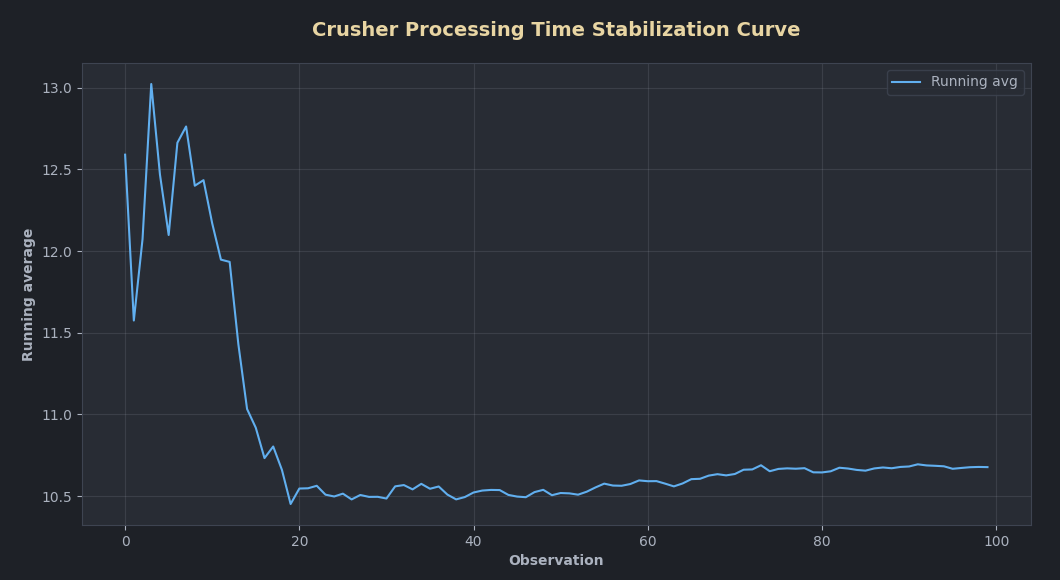
\includegraphics[width=0.7\linewidth]{stabilization-curve.png}
	\end{exampleblock}
\end{frame}

% ════════════════════════════════════════════════════════════
\section{\textbf{Pregunta 3:} Algoritmo Congruencial Lineal}
% ════════════════════════════════════════════════════════════

\sectionslide{Pregunta 3}{Generación de Variables Aleatorias (ACL)}

\begin{frame}{P3 · Ecuación Recursiva}
	\begin{block}{Algoritmo Congruencial Lineal}
		\[
			X_{i+1} = (a\,X_i + c)\;\operatorname{mod}(m)
			\qquad
			r_i = \frac{X_i}{m-1}
		\]
		Parámetros: semilla $X_0$, multiplicador $a$, constante $c$, módulo $m$
		(todos enteros $> 0$).
	\end{block}
	\vspace{0.25cm}
	\centering\footnotesize
	\renewcommand{\arraystretch}{1.3}
	\begin{tabular}{ccccc}
		\toprule
		$i$ & $X_i$ & $a\,X_i + c$ & $X_{i+1} = \operatorname{mod}(\cdot, m)$ & $r_i = X_i/(m-1)$ \\
		\midrule
		0   & $X_0$ &              &                                          & —                 \\
		1   &       &              &                                          &                   \\
		2   &       &              &                                          &                   \\
		3   &       &              &                                          &                   \\
		4   &       &              &                                          &                   \\
		5   &       &              &                                          &                   \\
		\bottomrule
	\end{tabular}
	\par\vspace{0.15cm}
	\textit{(Completar con los parámetros dictados en pizarra)}
\end{frame}

% ════════════════════════════════════════════════════════════
\section{\textbf{Pregunta 4:} Prueba de Medias}
% ════════════════════════════════════════════════════════════

\sectionslide{Pregunta 4}{Validación Estadística — Prueba de Medias}

\begin{frame}{P4 · Hipótesis y Límites de Aceptación}
	\begin{columns}[T]
		\column{0.48\linewidth}
		\begin{alertblock}{Hipótesis}
			\[
				H_0: \mu = 0.5 \quad \text{vs} \quad H_1: \mu \neq 0.5
			\]
			\[
				\bar{r} = \frac{1}{n}\sum_{i=1}^{n} r_i
			\]
		\end{alertblock}
		\vspace{0.3cm}
		\begin{block}{Promedio Muestral}
			\[
				\bar{r} = \frac{\ldots}{\ldots} = \boxed{\ldots}
			\]
		\end{block}
		\column{0.48\linewidth}
		\begin{block}{Límites de Aceptación}
			\[
				LI = 0.5 - Z_{\alpha/2}\,\frac{1}{\sqrt{12n}}
			\]
			\[
				LS = 0.5 + Z_{\alpha/2}\,\frac{1}{\sqrt{12n}}
			\]
			Con $Z_{\alpha/2} = \ldots$ (tabla normal estándar).
		\end{block}
		\vspace{0.2cm}
		\begin{exampleblock}{Conclusión}
			\footnotesize
			Como $\bar{r} \in [LI,\,LS]$, \textbf{no se rechaza} $H_0$:\\
			el generador es imparcial.
		\end{exampleblock}
	\end{columns}
\end{frame}

% ════════════════════════════════════════════════════════════
\section{\textbf{Pregunta 5:} Prueba de Varianza}
% ════════════════════════════════════════════════════════════

\sectionslide{Pregunta 5}{Validación Estadística — Prueba de Varianza}

\begin{frame}{P5 · Prueba Chi-Cuadrada (Varianza)}
	\begin{columns}[T]
		\column{0.48\linewidth}
		\begin{alertblock}{Hipótesis}
			\[
				H_0: \sigma^2 = \tfrac{1}{12} \quad \text{vs} \quad
				H_1: \sigma^2 \neq \tfrac{1}{12}
			\]
			\[
				V(r) = \frac{\sum(r_i - \bar{r})^2}{n-1} = \boxed{\ldots}
			\]
		\end{alertblock}
		\column{0.48\linewidth}
		\begin{block}{Límites Chi-Cuadrada}
			\[
				LI = \frac{\chi^2_{(1-\alpha/2),\,n-1}}{12(n-1)}
			\]
			\[
				LS = \frac{\chi^2_{\alpha/2,\,n-1}}{12(n-1)}
			\]
		\end{block}
	\end{columns}
	\vspace{0.35cm}
	\begin{exampleblock}{Conclusión estadística}
		\footnotesize
		Si $V(r) \in [LI,\,LS]$, \textbf{no se rechaza} $H_0$: la dispersión del
		generador es estadísticamente uniforme. En caso contrario se rechaza.
	\end{exampleblock}
	\result{$V(r) = \ldots$ \quad $LI = \ldots$ \quad $LS = \ldots$}
\end{frame}

% ════════════════════════════════════════════════════════════
\section{\textbf{Pregunta 6:} Prueba de Uniformidad Chi-Cuadrada}
% ════════════════════════════════════════════════════════════

\sectionslide{Pregunta 6}{Uniformidad — Prueba Chi-Cuadrada}

\begin{frame}{P6 · Estadístico de Prueba}
	\begin{block}{Hipótesis y formulación}
		\[
			H_0: r_i \sim U(0,1)
			\qquad
			m = \lceil\sqrt{n}\rceil \text{ subintervalos}
			\qquad
			E_i = \frac{n}{m}
		\]
		\[
			\chi^2_0 = \sum_{i=1}^{m} \frac{(E_i - O_i)^2}{E_i}
		\]
	\end{block}
	\vspace{0.2cm}
	\centering\footnotesize
	\renewcommand{\arraystretch}{1.3}
	\begin{tabular}{ccccc}
		\toprule
		Subintervalo                               & Límites       & $O_i$    & $E_i$    & $(E_i-O_i)^2/E_i$ \\
		\midrule
		1                                          & $[0.0,\;0.x)$ &          &          &                   \\
		2                                          & $[0.x,\;0.y)$ &          &          &                   \\
		$\vdots$                                   & $\vdots$      & $\vdots$ & $\vdots$ & $\vdots$          \\
		$m$                                        & $[0.z,\;1.0)$ &          &          &                   \\
		\midrule
		\multicolumn{4}{r}{\bfseries $\chi^2_0 =$} &                                                         \\
		\bottomrule
	\end{tabular}
	\par\vspace{0.2cm}
	\begin{exampleblock}{}
		\centering\footnotesize
		Si $\chi^2_0 < \chi^2_{\alpha,\,m-1}$ (tabla) $\Rightarrow$
		\textbf{no se rechaza} $H_0$: uniformidad confirmada.
	\end{exampleblock}
\end{frame}

% ── Cierre ───────────────────────────────────────────────────
{
\setbeamertemplate{headline}{}
\setbeamertemplate{footline}{}
\begin{frame}[plain]
	\begin{tikzpicture}[remember picture, overlay]
		\fill[darkblue] (current page.south west) rectangle (current page.north east);
		\node[font=\Huge\bfseries\color{purewhite}, align=center]
		at (current page.center) {Gracias por su atención};
	\end{tikzpicture}
\end{frame}
}

\end{document}
